\documentclass[a4paper,10pt]{article}
\usepackage[margin=1in]{geometry}
\usepackage[utf8]{inputenc}
\usepackage{graphicx}
\usepackage{enumitem} % enum styles
\usepackage{color}
\usepackage{hyperref}
\usepackage{subfig}
\usepackage{booktabs}
\usepackage{multirow}

\setitemize{itemsep=1pt,parsep=2pt,topsep=8pt,partopsep=0pt, label=-}
\setenumerate{itemsep=1pt,parsep=2pt,topsep=2pt,partopsep=0pt}

\usepackage{listings}
\lstset{language=C}

%\lstMakeShortInline[columns=fixed]|


\definecolor{mygreen}{rgb}{0,0.6,0}
\definecolor{mygray}{rgb}{0.5,0.5,0.5}
\definecolor{mymauve}{rgb}{0.07,0.31,0.35}

\lstset{
  frameround=fttt,
  language=C,
  numbers=left,
  breaklines=true,
  %breakatwhitespace=true,
  basicstyle=\ttfamily\color{black},
  keywordstyle=\color{mymauve}\bfseries,
  numberstyle=\color{black},
  stringstyle=\color{orange},
  commentstyle=\color{grey},
  identifierstyle=\color{black},
  postbreak=\mbox{\textcolor{red}{$\hookrightarrow$}\space},
  literate={\_}{}{0\discretionary{\_}{}{\_}}%
}

\usepackage{paratype}
\renewcommand*\familydefault{\sfdefault} %% Only if the base font of the document is to be sans serif
\usepackage[T1]{fontenc}
\renewcommand{\baselinestretch}{1.12}

\usepackage{fancyhdr}
\pagestyle{fancy}
\fancyhf{}
\rhead{\leftmark}
\lhead{Fibers}
\cfoot{\thepage}

\title{
  \huge \textbf{Fibers} \\
  \Large Final Project Essay \\
  \noindent \rule{9cm}{0.2pt} \\
  \large Advanced Operating Systems and Virtualization \\
  \large \textit{Sapienza University of Rome}
}
\author{
  Gabriele Proietti Mattia \\ 1645351 \and Alexandru Daniel Tufa \\ 1628927
}
\date{\today\ (A.Y. 17/18)}


\begin{document}
\maketitle

%\tableofcontents

\section{Introduction}
 Fibers are the Windows kernel-level implementation of User-Level Threads. To perfectly understand them, let’s see the difference with kernel level threads. Kernel-Level Threads are implemented when the Operating System manages the execution aspect of a process, which is separated into threads. These threads managed by the OS are called kernel-level threads or lightweight processes. The advantages here are that the kernel has full knowledge of all threads, meaning that it can optimize them, for example by assigning more time to a process having a large number of threads rather than a process with a small number of threads. On the other side, kernel-level threads are slow and inefficient, requiring an additional data structure (Thread Control Block) for each thread to maintain information about them. This results in a significant overhead.

 In order to make the programs using threads faster, they should be implemented at user level, where User-Level Threads are managed entirely by the user-level library. This results in the kernel knowing nothing about user-level threads and it will manage them as if they were single-threaded processes. In this way, each user-level thread is represented by its set of registers and stack. This methodology allows for offering threads to an Operating System that could not support threads and don’t require the modification of the OS for supporting them; has simple representation and management and can be considered fast and efficient since thread switching is not much more expensive than a procedure call.

 With this project we try to implement User-Level Threads through the use of the kernel. As a guide we have used the information provided by Windows, which states that a fiber is a unit of execution that must be manually scheduled by the application. This means that a fiber is not preemptively scheduled, but one schedules a fiber by switching to it from another fiber. This doesn’t mean or imply that one application using fibers doesn’t make use of normal threads. When using fibers, the fiber assumes the identity of the thread that runs it, implying that if a thread running fibers is preempted, its currently running fiber is preempted but remains selected. This grants the possibility for handling concurrency in a much more fine-grained manner since the user can establish the schedule of the fibers by himself and not assign this task to a system that does this in a non-deterministic fashion.
 In order to start using fibers and make a thread fiber-enabled, it must call the \lstinline{ConvertThreadToFiber} function which:
 \begin{itemize}
   \item makes the thread into a fiber;
   \item gives this fiber the capability of creating other fibers;
 \end{itemize}
 To create a new fiber from an existing one, the CreateFiber function is to be used. The needed data for a fiber to run is:
 \begin{itemize}
   \item function to execute, which is called the fiber function;
   \item stack size;
   \item fiber data, input for the fiber function;
 \end{itemize}

 Once a fiber has been newly created, the user can switch to it by using the SwitchToFiber function.
 To store information related to a precise fiber, the user can use the Fiber Local Storage which, through the use of the FLS functions (\lstinline{FlsAlloc}, \lstinline{FlsFree}, \lstinline{FlsGetValue}, \lstinline{FlsSetValue}), allows for the manipulation of values associated to single fibers.

\section{Design Choices}
 The project consists of two sides: the kernel module that represents the kernel side (that we will call \textit{fiber module}) and the library (that we will call \texttt{fiber library}) that represents the userspace side of the framework. This kind of approach is the simplest one for implementing system calls: the module exposes a device in /dev/fiber and whenever the library needs to call a function exposed by the module it uses the system call ioctl, that given the fiber device file and a function integer id, it performs the call as it was a standard system call.

 This is the general approach that we used for implementing the fiber logic. Obviously the library and module needs different kind of data to be stored and they have different workflows, for this reason in the following sections we will see them in detail.

\subsection{Kernel Module}
\subsubsection{Data Structures}\label{subsubsec:kern-datas}
  We chose to represent a fiber with the following attributes:
  \begin{itemize}
    \item \lstinline{int id}: unique for each fiber, that we’ll reference also as fid (fiber id);
    \item \lstinline{struct pt_regs registers}: snapshot of the CPU registers. The internal state of a fiber is represented through the content in the registers. To change the execution flow, thus changing from one fiber to another, we swap the registers. The most important ones here are the instruction pointer (\texttt{IP}) and stack pointer (\texttt{SP});
    \item \lstinline{fiber_state_t state}: an enumeration that represents the current state of fiber \lstinline{RUNNING} or \lstinline{IDLE};
    \item \lstinline{unsigned long entry point}: starting function of the fiber
    \item \lstinline{unsigned created_by}: pid of the thread that created the fiber;
    \item \lstinline{unsigned run_by}: pid of the thread that is currently running this fiber. If no thread is running it, we recur to the default value of -1;
    \item \lstinline{unsigned success_activations} number of times the fiber has been switch to successfully;
    \item \lstinline{unsigned failed_activations} number of times the fiber activation failed, for example when we try to switch to an already running fiber;
    \item \lstinline{unsigned long total_time}: total running time of the fiber
    \item \lstinline{struct timespec time_last_switch}: time of when the last switch from one fiber to another occurred;
    \item \lstinline{fiber_fls_t local_storage}: a structure that represents the fiber local storage.
  \end{itemize}

  To correctly access and handle fibers, we use two lists:
  \begin{itemize}
    \item \lstinline{fibered_processes_list_t fibered_processes_list}: a list of processes which are fiber-enabled. Each fibered\_process is identified by its tgid and contains a list of fibers
    \item \lstinline{fibers_list_t fibers_list}: a list of fibers for each fibered\_process
  \end{itemize}

  To manage the fiber local storage, for each fiber we declare:
  \begin{itemize}
    \item an array of an established maximum dimension
    \item a bitmap which allows for handling in a fast and efficient way the allocation, freeing, setting and getting of values
  \end{itemize}

\subsubsection{Workflows}
  \paragraph{Converting a standard thread to a fiber}
    The first function that need to be called for starting using fibers is \lstinline{ConvertThreadToFiber}, since only a thread that is a fiber can create other fibers and switch to them. When a thread of a process calls for the first time \lstinline{ConvertThreadToFiber} we say that the process becomes \textit{fiber-enabled} or \textit{fibered}, meaning that we have added it our list of fibered processes \lstinline{fibered_processes_list_t}. Therefore \lstinline{ConvertThreadToFiber} needs to add the process to the list and then create an entry in the fibers list of the same process, representing the thread that has been converted to a fiber.

  \paragraph{Creating fibers}
    At this point the thread can call any other function offered by the module. The function \lstinline{CreateFiber} creates a brand new fiber node to the list of fibers of the current process. The kernel module expects the library to pass a series of parameters for the fiber, as the \textbf{memory address} of the stack, the address of the \textbf{starting function} of the fiber and also a pointer to its \textbf{arguments}. These parameters are used for configuring the registers that will be restored in the CPU when some thread will switch to that fiber. In particular we set Stack Pointer (\texttt{SP}) and the Stack Base Pointer (\texttt{BP}) to the memory address of the stack passed by the library, Intruction Pointer (\texttt{IP}) to the address of the starting function of the fiber and Destrination Index (\texttt{DI}) to arguments’ memory address. Every other parameter is then initialized, as the activation count, the total time, the state, the id and so on (see Section~\ref{subsubsec:kern-datas}).

  \paragraph{Switching to a fiber}
    The function that makes a fiber running is \lstinline{SwitchToFiber}. Any fiber can switch to any other non-running fiber\footnote{If a currently running fiber tries to switch to a running fiber the \lstinline{failed_activation} counter is incremented for the requested fiber}. This function is achieved by actually realizing a context switch between fibers. The current state of the CPU of the current fiber is saved in the fiber data structure (describe in Section~\ref{subsubsec:kern-datas}), and then we restore the CPU state (including the fpu registers) of the requested fiber thus changing the flow of the execution of the current thread. In this moment also other metadata are set: the current fiber \lstinline{state} is set to \texttt{IDLE}, while the requested fiber state is set to \texttt{RUNNING} and updated with the \texttt{pid} of the current thread, then we also update the total running time of the left fiber.

  \paragraph{The Fiber Local Storage (FLS)}
    To be able to use the Fiber Local Storage the user has to call \lstinline{FlsAlloc}. In this way the system will give, to the fiber which called the function, a way to access its requested space. In particular, \lstinline{FlsAlloc} returns the index of the first free slot of fiber space\footnote{The size of every slot is \lstinline{sizeof(unsigned long)}}. This index can be then used to store a value, by using the function \lstinline{FlsSetValue}, and also for retrieving it, through the function \lstinline{FlsGetValue}. To check if the index is a valid one, the kernel uses the functionalities offered by the bitmap. When the space associated with a certain index is no longer needed, it’s enough for the user to call \lstinline{FlsFree} and passing the not-needed-anymore index and the system will clear its position in the bitmap.

\subsubsection{\texttt{\/proc} filesystem}\label{subsubsec:kern-procfs}
  The implementation of the \texttt{/proc} specification does not follow the canonical strategy that is requested for creating directory and files in the \texttt{procfs}. This because directories that can be found in \lstinline{/proc/<PID>} are not \textit{statically} created, on the contrary, they are generated ``on the fly'', only when they are requested, mainly due to optimization reasons\footnote{A process can, for example, live for only few milliseconds and as a consequence it would be not efficient to build an entire directory tree}. As a consequence, for achieveing the specification we needed to design a sort of ``hacking plan'' aimed to add the desired folder \lstinline{/proc/<PID>/fibers}.

  First of all, we must know that the set of files and directories that are displayed in \lstinline{/proc/<PID>} are described by an array of \lstinline{struct pid_entry}, called \lstinline{tgid_base_stuff}~\cite{kern_tgid_base_stuff}. This array has fixed size, and every entry is filled so we have not spare slots that can be filled, therefore the only way to add things to it is to create an ``hook'' towards that functions that use it. In particular, found that \lstinline{proc_pident_readdir} takes as input \lstinline{tgid_base_stuff} and it instantiates every entry in the array, thus allowing them to be accessed.

  A valid way for replacing the address of a function used by the kernel is using the \lstinline{ftrace} subsystem. So we created a customized version of the function \lstinline{proc_pident_readdir} that before calling the real function it simply adds one entry in the array of \lstinline{struct pid_entry} passed as parameter\footnote{Since the \lstinline{proc_pident_readdir} function is also called when accessing subfolders in \lstinline{/proc/<PID>} we firstly check if the name of the current directory is a PID, otherwise the fallback to the original version of the function} (obviously only if the process is \textit{fibered}). This particular entry of array represents the \texttt{fibers} directory.

  The next step of the implementation is aimed to allow the user to navigate the \texttt{fibers} folder, more specifically we wanted to have a file for every created fiber, like \lstinline{/proc/<PID>/fibers/<FID>} where \texttt{FID} is actually the fiber id. For implementing this, we must admit that \texttt{fibers} is, after all, a directory of the VFS, even if it is wrapped in a \lstinline{pid_entry} structure. Therefore we only needed to implement the standard functions:
  \begin{itemize}
    \item \lstinline{iterate_shared()}~\cite{kern_file_ops_iterate} in the \lstinline{struct file_operations}, whose purpose is to instantiate the actual items of a directory. We mapped it to our custom function \lstinline{proc_fibers_dir_readdir()};
    \item \lstinline{lookup()}~\cite{kern_inode_ops_lookup} in the \lstinline{struct inode_operations} whose purpose is to retrieve the desired item inside a directory. We mapped it to our custom function \lstinline{proc_fibers_dir_lookup()}.
  \end{itemize}
  Both \lstinline{proc_fibers_dir_readdir()} and \lstinline{proc_fibers_dir_lookup()} takes as input an array of \lstinline{pid_entry} (like \lstinline{tgid_base_stuff}) but now this array will be requested to have an entry, representing a regular file, for each created fiber. So we implemented a function for this purpose, \lstinline{generate_fibers_dir_stuff()}, that given the directory automatically generates an array of \lstinline{pid_entry} in which every file has as name the id of the fiber and its \lstinline{read()} function is associated to the one that prints all the needed information\footnote{This last part is the only one that is compliant to the standard strategy of creating regular files in \texttt{procfs}}.


\subsection{Userspace Library}

\subsubsection{Data Structures}
  The information needed for representing fibers in the library is less than the one needed in the kernel. Here we use the following attributes for handling them:
  \begin{itemize}
    \item \lstinline{stack_size}: size of the stack that will be used by the execution flow of the fiber
    \item \lstinline{stack_addr}: the stack starting address allocated by the library
    \item \lstinline[language={}]{function}: the function pointer passed by the user, that will be the starting point of the fiber
    \item \lstinline{function_args}: arguments for the fiber function
  \end{itemize}

  The purpose of this data structure is to avoid to call the kernel module when is not needed, for example when switching to a fiber is useless to call the module if the requested fiber does not exists, indeed we first check if the fiber exists in our data structure and if not we avoid calling ioctl on the fiber device.

\subsubsection{Workflows}\label{subsubsec:lib-works}
  The library acts as an intermediate between the user and the kernel, more precisely our module. The means of communication is offered by the ioctl function.

\section{Implementation Details}
\subsection{Worktrees}
  The \textbf{kernel module} worktree is made up the following source files in src/:
  \begin{itemize}
    \item \lstinline{fiber.c} represents the module entry point, so its purpose is to initialize of the subparts, like the \lstinline{device} and the \lstinline{procfs};
    \item \lstinline{device.c} it's focused on the creation and the management of the fiber device in \lstinline{/dev/fiber}, and as a consequence of all what regards the dispatch of the \lstinline{ioctl} commands;
    \item \lstinline{proc.c} represents the \lstinline{procfs} part of the module, the one that gives life to \lstinline{/proc/<PID>/fibers} (see Section~\ref{subsubsec:kern-procfs});
    \item \lstinline{core.c} implements all the services exposed by the module and also retains the main data structure used for storing all the fibers information.
  \end{itemize}
  In the \lstinline{include} folder we have an header file for every code file, except for:
  \begin{itemize}
    \item \lstinline{utils.h} contains mainly definition of macros that we use to scroll kernel linked lists and hash tables that we use as database of our module;
    \item \lstinline{ioctlcmd.h} represent the interconnection point between the module and the library since this file is shared between them. Its purpose is to store information about \lstinline{ioctl} commands identifiers and common data structures, as the \lstinline{fiber_params_t}\footnote{Whose purpose is to tell the kernel, from the library, all the information about a new fiber as: stack address, entry point and so on.}.
    \item \lstinline{common.h} it's a general configuration file imported by all code files. It tells wether to use hash tables or linked list (for the fibered processes data structure), it specifies the dimension of the FLS storage and other parameters.
  \end{itemize}

  The \textbf{library} worktree is made up by:
  \begin{itemize}
    \item \lstinline{core.c} implements all the set of userspace callable function, directly mapped to \lstinline{ioctl} commands (see Section~\ref{subsubsec:lib-works}) and the data structure that represents all the fibers managed by a process.
    \item \lstinline{fiber_example.c} contains a little running example mainly used for testing the library and the module functionality.
  \end{itemize}
  and as headers:
  \begin{itemize}
    \item \lstinline{fiber.h} contains the prototype of all the set of the functions requested by the specification of the project, as: \lstinline{CreateFiber}, \lstinline{SwitchToFiber}, and so on;
    \item \lstinline{list.h} contains the userspace implementation of the linked list data structures used in the kernel (it consists of only macros, all the architecture-dependent optimization has been removed~\cite{klists}).
    \item \lstinline{utils.h} contains utilities for accessing linked lists, as in the kernel module;
    \item \lstinline{common.h} general configuration file.
  \end{itemize}


\subsection{OS \& tools}
  This project has been developed and tested to be working with the following environment parameters:
  \begin{itemize}
    \item \textbf{Linux Distros}: Fedora, Arch Linux, Debian 9 and Ubuntu 18.04;
    \item \textbf{Linux Kernel}: \lstinline{v4.14.38};
    \item \textbf{Compiling Suite}: \lstinline{gcc} (\lstinline{v7.3.0/1});
    \item \textbf{IDE}: Visual Studio Code.
  \end{itemize}

\section{Benchmark assessment}

\subsection{2 cores virtual machine}
 \begin{table}[ht!]
  \centering
  \begin{tabular}{@{}lllllllllll@{}}
  \toprule
    &  & \multicolumn{9}{c}{\textit{\textbf{Number of Fibers}}} \\ \midrule
    &  & \textbf{3} & \textbf{5} & \textbf{7} & \textbf{9} & \textbf{11} & \textbf{13} & \textbf{15} & \textbf{17} & \textbf{19} \\
  \multirow{9}{*}{\rotatebox[origin=c]{90}{\textit{\textbf{Number of processes}}}} & \textbf{1} & 0.324 & 0.329 & 0.324 & 0.331 & 0.335 & 0.359 & 0.341 & 0.338 & 0.332 \\
    & \textbf{3} & 0.977 & 0.977 & 1.029 & 0.976 & 1.122 & 1.148 & 1.265 & 1.18 & 1.195 \\
    & \textbf{5} & 1.629 & 2.101 & 1.634 & 1.646 & 2.677 & 2.499 & 1.748 & 2.642 & 2.215 \\
    & \textbf{7} & 2.233 & 2.506 & 3.502 & 3.474 & 3.298 & 3.471 & 4.186 & 4.152 & 3.857 \\
    & \textbf{9} & 2.904 & 3.818 & 3.423 & 5.237 & 5.014 & 4.817 & 5.398 & 5.613 & 5.728 \\
    & \textbf{11} & 3.557 & 4.273 & 6.201 & 5.928 & 6.066 & 6.621 & 6.688 & 6.916 & 6.913 \\
    & \textbf{13} & 5.608 & 5.226 & 6.566 & 7.736 & 6.995 & 7.972 & 8.008 & 8.149 & 7.732 \\
    & \textbf{15} & 6.141 & 7.906 & 6.999 & 9.07 & 9.198 & 9.329 & 9.386 & 9.738 & 8.884 \\
    & \textbf{17} & 7.298 & 8.613 & 9.498 & 9.543 & 9.527 & 10.125 & 10.505 & 9.672 & 10.855 \\ \bottomrule
  \end{tabular}
  \caption{Mean fiber execution time (in seconds) in a machine with 2 cores by using hash table}
  \label{tab:2cores-hashes}
\end{table}

 \begin{table}[ht!]
  \centering
  \begin{tabular}{@{}lllllllllll@{}}
  \toprule
    &  & \multicolumn{9}{c}{\textit{\textbf{Number of Fibers}}} \\ \midrule
    &  & \textbf{3} & \textbf{5} & \textbf{7} & \textbf{9} & \textbf{11} & \textbf{13} & \textbf{15} & \textbf{17} & \textbf{19} \\
  \multirow{9}{*}{\rotatebox[origin=c]{90}{\textit{\textbf{Number of processes}}}} & \textbf{1} & 0.329 & 0.338 & 0.326 & 0.351 & 0.331 & 0.328 & 0.328 & 0.342 & 0.335 \\
    & \textbf{3} & 0.978 & 1.202 & 0.961 & 1.003 & 0.997 & 1.014 & 0.98 & 1.199 & 1.055 \\
    & \textbf{5} & 1.642 & 1.621 & 1.879 & 2.327 & 2.346 & 2.072 & 2.339 & 2.263 & 2.114 \\
    & \textbf{7} & 2.261 & 3.42 & 3.349 & 3.986 & 3.468 & 4.294 & 4.138 & 4.261 & 4.263 \\
    & \textbf{9} & 2.876 & 3.971 & 4.65 & 4.379 & 5.137 & 5.48 & 5.573 & 5.32 & 5.639 \\
    & \textbf{11} & 3.775 & 5.675 & 5.481 & 6.084 & 6.094 & 6.621 & 6.518 & 6.889 & 6.463 \\
    & \textbf{13} & 4.194 & 5.911 & 7.315 & 6.546 & 7.525 & 7.978 & 7.166 & 7.713 & 7.169 \\
    & \textbf{15} & 6.319 & 6.962 & 7.527 & 6.743 & 8.923 & 8.651 & 9.091 & 9.467 & 9.304 \\
    & \textbf{17} & 5.738 & 8.13 & 9.51 & 10.084 & 10.245 & 9.369 & 10.205 & 10.282 & 10.716 \\ \bottomrule
  \end{tabular}
  \caption{Mean fiber execution time (in seconds) in a machine with 2 cores by using linked list}
  \label{tab:2cores-linked}
  \end{table}

 \begin{figure}[ht!]
   \centering
   \begin{minipage}{0.45\textwidth}%
     \centering
     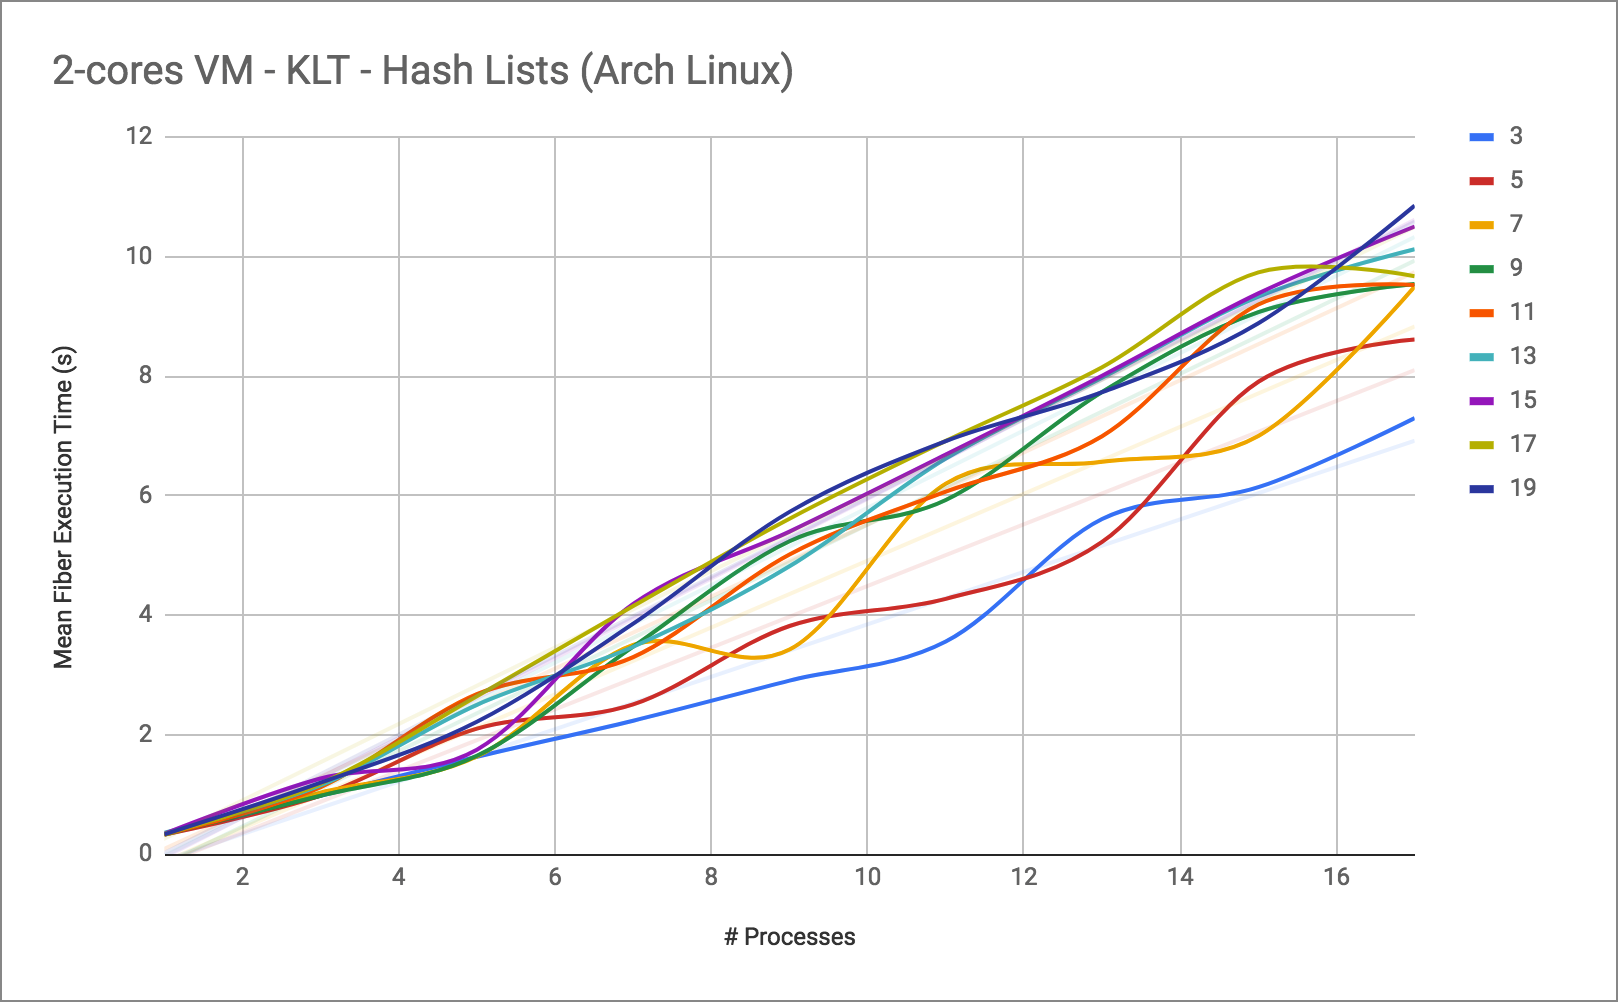
\includegraphics[width=\textwidth]{imgs/bench-2cores-hash}
     \caption{Fiber modules using hash table}
     \label{fig:2figsA}
   \end{minipage}%
   \qquad
   \begin{minipage}{0.45\textwidth}%
     \centering
     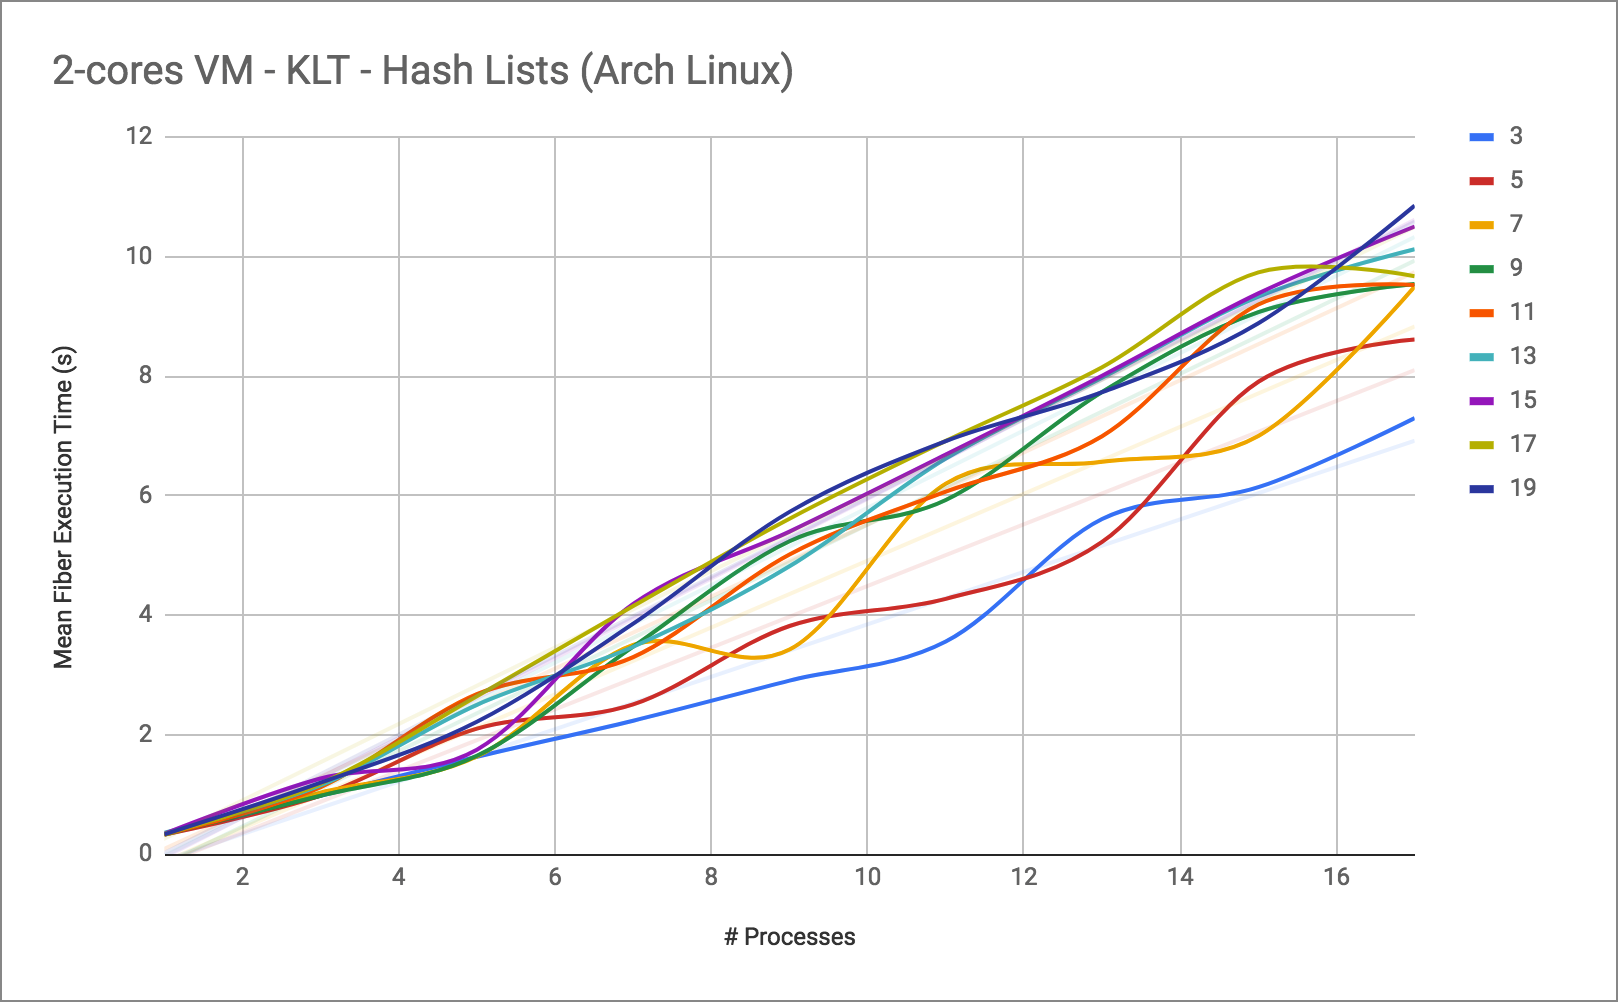
\includegraphics[width=\textwidth]{imgs/bench-2cores-hash}
     \caption{Fiber modules using linked list}
     \label{fig:2figsB}%
   \end{minipage}%
   \caption{Plot of mean fiber execution times on a machine with 2 cores}
 \end{figure}


 \subsection{4 cores virtual machine}

 \begin{table}[ht!]
  \centering
  \begin{tabular}{@{}lllllllll@{}}
  \toprule
   &  & \multicolumn{7}{c}{\textit{\textbf{Number of Fibers}}} \\ \midrule
   &  & \textbf{5} & \textbf{7} & \textbf{9} & \textbf{11} & \textbf{13} & \textbf{15} & \textbf{17} \\
  \multirow{9}{*}{\rotatebox[origin=c]{90}{\textit{\textbf{Number of processes}}}} & \textbf{1} & 0.546 & 0.702 & 0.56 & 0.557 & 0.401 & 0.377 & 0.377 \\
   & \textbf{3} & 1.8 & 2.11 & 1.459 & 1.627 & 1.127 & 1.127 & 1.164 \\
   & \textbf{5} & 2.411 & 2.936 & 3.225 & 3.26 & 1.924 & 2.185 & 1.886 \\
   & \textbf{7} & 3.997 & 4.611 & 4.787 & 4.488 & 3.102 & 3.189 & 3.08 \\
   & \textbf{9} & 5.88 & 4.737 & 4.646 & 5.78 & 4.534 & 4.618 & 4.615 \\
   & \textbf{11} & 5.666 & 5.324 & 5.478 & 6.78 & 6.096 & 6.148 & 5.878 \\
   & \textbf{13} & 7.145 & 6.337 & 7.905 & 10.941 & 6.668 & 7.299 & 6.568 \\
   & \textbf{15} & 7.33 & 8.712 & 10.076 & 11.885 & 8.985 & 8.422 & 7.454 \\
   & \textbf{17} & 9.273 & 9.922 & 10.868 & 12.939 & 10.201 & 9.865 & 10.699 \\ \bottomrule
  \end{tabular}
  \caption{Mean fiber execution time (in seconds) in a machine with 4 cores by using hash table}
  \label{tab:4cores-hash}
  \end{table}

\begin{table}[ht!]
  \centering
  \begin{tabular}{@{}lllllllll@{}}
  \toprule
    &  & \multicolumn{7}{c}{\textit{\textbf{Number of Fibers}}} \\ \midrule
    &  & \textbf{5} & \textbf{7} & \textbf{9} & \textbf{11} & \textbf{13} & \textbf{15} & \textbf{17} \\
  \multirow{9}{*}{\rotatebox[origin=c]{90}{\textit{\textbf{Number of processes}}}} & \textbf{1} & 0.37 & 0.418 & 0.54 & 0.372 & 0.376 & 0.414 & 0.49 \\
    & \textbf{3} & 1.316 & 1.245 & 1.323 & 1.168 & 1.768 & 1.301 & 1.313 \\
    & \textbf{5} & 2.003 & 2.01 & 1.9 & 2.196 & 2.304 & 2.196 & 1.928 \\
    & \textbf{7} & 2.737 & 2.903 & 2.877 & 2.871 & 2.79 & 3.079 & 3.552 \\
    & \textbf{9} & 3.468 & 3.422 & 3.504 & 3.798 & 4.266 & 4.199 & 4.407 \\
    & \textbf{11} & 4.996 & 4.313 & 5.575 & 7.142 & 6.99 & 5.575 & 5.649 \\
    & \textbf{13} & 5.212 & 5.353 & 5.864 & 7.283 & 7.523 & 8.007 & 6.571 \\
    & \textbf{15} & 6.842 & 6.485 & 7.071 & 10.657 & 14.036 & 11.248 & 8.593 \\
    & \textbf{17} & 8.36 & 15.222 & 10.682 & 13.535 & 15.929 & 16.13 & 15.145 \\ \bottomrule
  \end{tabular}
  \caption{Mean fiber execution time (in seconds) in a machine with 4 cores by using linked list}
  \label{tab:4cores-linked}
  \end{table}

 \begin{figure}[ht!]
   \centering
   \begin{minipage}{0.45\textwidth}%
     \centering
     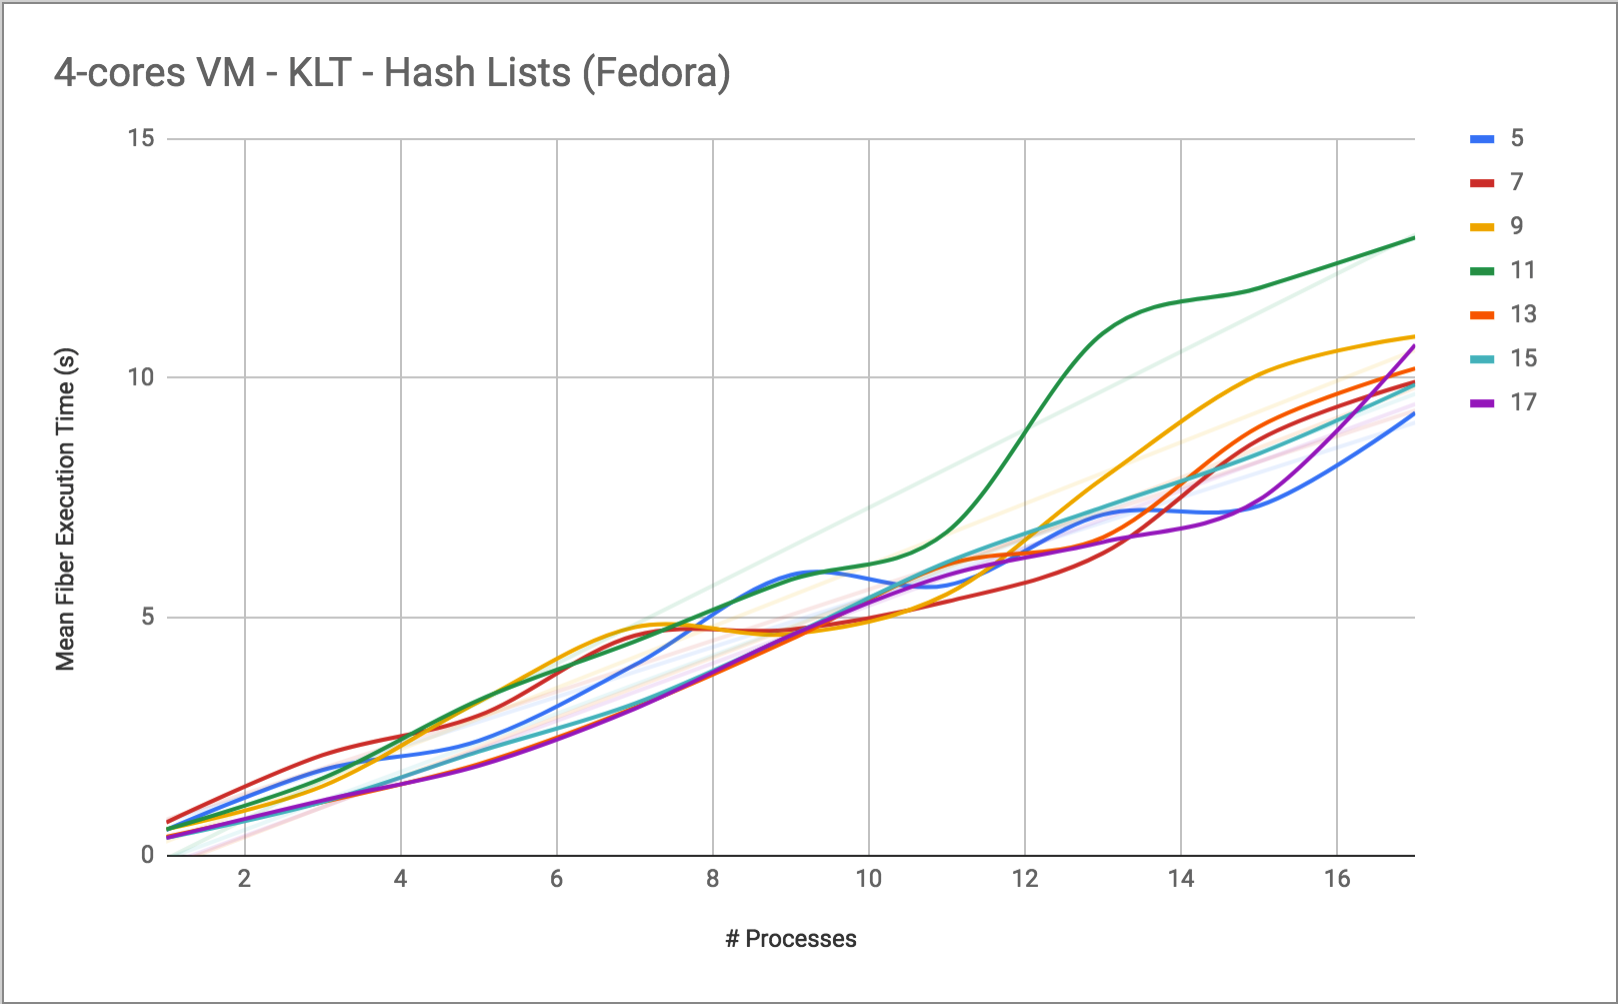
\includegraphics[width=\textwidth]{imgs/bench-4cores-hash}
     \caption{Fiber modules using hash lists}
     \label{fig:2figsA}
   \end{minipage}%
   \qquad
   \begin{minipage}{0.45\textwidth}%
     \centering
     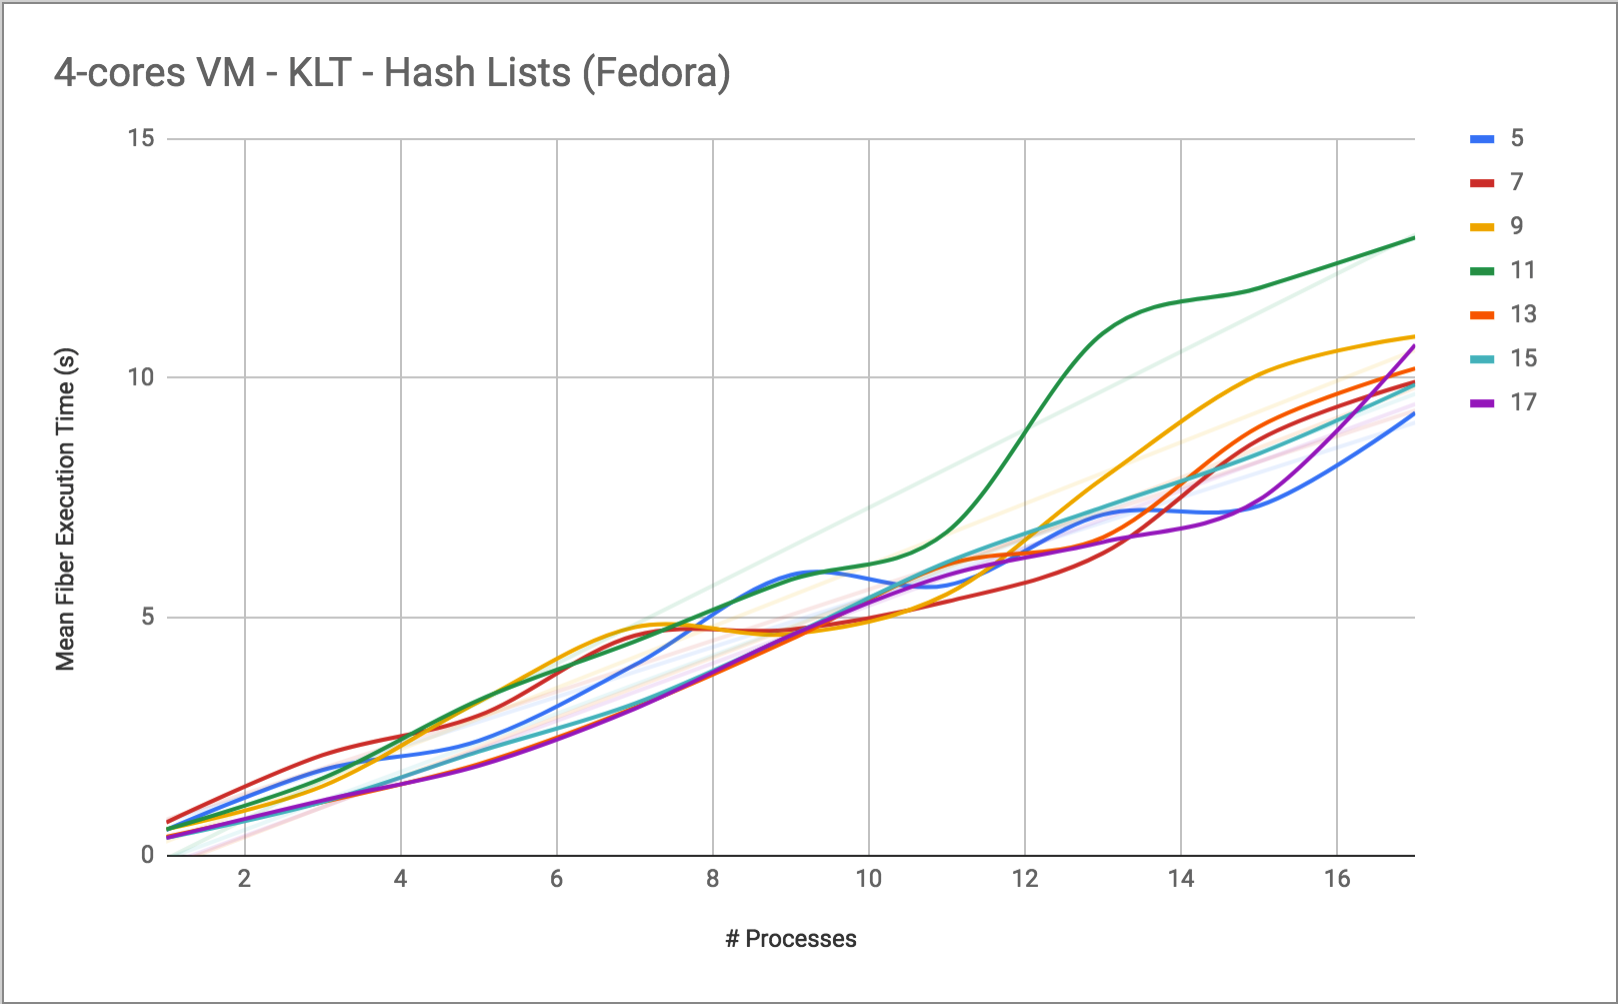
\includegraphics[width=\textwidth]{imgs/bench-4cores-hash}
     \caption{Fiber modules using linked lists}
     \label{fig:2figsB}%
   \end{minipage}%
   \caption{Plot of mean fiber execution times on a machine with 4 cores}
 \end{figure}

 \begin{thebibliography}{9}

   \bibitem{kern_tgid_base_stuff}
   \lstinline{tgid_base_stuff}, \lstinline{/fs/proc/base.c#2921}, Linux Kernel v4.14.38.

   \url{https://elixir.bootlin.com/linux/v4.14.38/source/fs/proc/base.c#L2921}

   \bibitem{kern_proc_pident_readdir}
   \lstinline{proc_pident_readdir}, \lstinline{/fs/proc/base.c#2489}, Linux Kernel v4.14.38.

   \url{https://elixir.bootlin.com/linux/v4.14.38/source/fs/proc/base.c#L2489}

   \bibitem{kern_file_ops_iterate}
   \lstinline{file_operations::iterate_shared}, \lstinline{/include/linux/fs.h#1701}, Linux Kernel v4.14.38.

   \url{https://elixir.bootlin.com/linux/v4.14.38/source/include/linux/fs.h#L1701}

   \bibitem{kern_inode_ops_lookup}
   \lstinline{inode_operations::lookup}, \lstinline{/include/linux/fs.h#1734}, Linux Kernel v4.14.38.

   \url{https://elixir.bootlin.com/linux/v4.14.38/source/include/linux/fs.h#L1734}

   \bibitem{klists}
   Linux Kernel Linked List Explained, NYU University.

   \url{https://isis.poly.edu/kulesh/stuff/src/klist/}

 \end{thebibliography}

\end{document}